\documentclass{beamer}
\usepackage{tikz}
\usetikzlibrary{arrows.meta, positioning}
\usetheme{Rochester}

\title{TIPE 25/26 - Cycles et Boucles}
\author{GIL Dorian}
\subtitle{Méthode des tableaux : Optimisation pour des formules de la forme (?)}
\date{}

\begin{document}

\begin{frame}
\titlepage
\end{frame}

\begin{frame}{Sommaire}
\begin{enumerate}
    \item Présentation
    \item Implémentation
    \item Ce qui est à faire
\end{enumerate}
\end{frame}

\begin{frame}{Présentation}
    On souhaite prouver une formule dans la logique propositionelle :
    \begin{definition}[Méthode des tableaux]
        Méthode par laquelle on prouve une assertion $B$ ayant pour hypothèse $(A_n)$ en montrant
        que $\{A_1,\dots,A_n, \lnot B\}$ est insatisfaisable (Cela revient à montrer qu'une implication est vraie car sa négation ne peut être vraie).
    \end{definition}
    \pause
    \begin{itemize}
        \item On place $\lnot\phi$ dans la racine d'un arbre de déduction.
        \item On applique des règles $(R_x)$ à chaque branche de l'arbre
        \item Si in fine on trouve $a$ et $\lnot a$ dans une branche, alors $\phi$ est vrai
    \end{itemize}
    \pause
    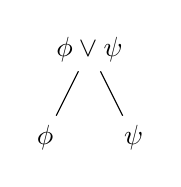
\begin{tikzpicture}[scale=0.75]
    \node {$\phi\lor\psi$}
        child {node {$\phi$}}
        child {node {$\psi$}};
    \end{tikzpicture}
    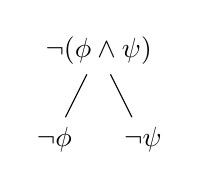
\begin{tikzpicture}[scale=0.75]
    \node {$\lnot(\phi\land\psi)$}
        child {node {$\lnot\phi$}}
        child {node {$\lnot\psi$}};
    \end{tikzpicture}
    \begin{tikzpicture}[scale=0.75]
    \node {$\lnot\lnot\phi$}
        child {node {$\phi$}};
    \end{tikzpicture}
    \begin{tikzpicture}[level distance=8mm]
    \node {$\phi\land\psi$}
        child {node {$\phi$} edge from parent }{
        child {node {$\psi$} edge from parent[draw=none]}};
    \end{tikzpicture}  
    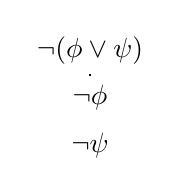
\begin{tikzpicture}[level distance=8mm,scale=0.75]
    \node {$\lnot(\phi\lor\psi)$}
        child {node {$\lnot\phi$} edge from parent }{
        child {node {$\lnot\psi$} edge from parent[draw=none]}};
    \end{tikzpicture}
    Les règles
\end{frame}




\begin{frame}{Analytic Tableau Example}
    \frametitle{Application of the Method of Analytic Tableau}

    % Define the logical formula
    \textbf{Formula:} $P \land (Q \lor R) \implies S$

    \vspace{1cm}

    % Start the tableau
    \begin{center}
    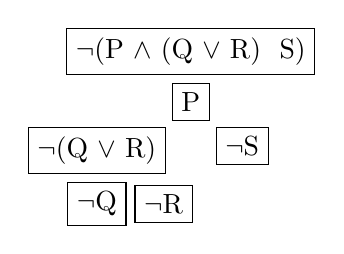
\begin{tikzpicture}[
        node distance=1mm,
        every node/.style={draw, rectangle, minimum width=2mm, minimum height=1mm},
        every edge/.style={->, thick}
    ]

    % Nodes
    \node (start) {$\lnot$(P $\land$ (Q $\lor$ R) $\implies$ S)};
    \node (negP) [below=of start] {P};
    \node (negQorR) [below left=of negP] {$\lnot$(Q $\lor$ R)};
    \node (negS) [below right=of negP] {$\lnot$S};
    
    \node (negQ) [below=of negQorR] {$\lnot$Q};
    \node (negR) [right=of negQ] {$\lnot$R};

    % Edges
    \path[every node/.style={sloped, anchor=center}]
        (start) edge (negP)
        (negP) edge (negQorR)
        (negP) edge (negS)
        (negQorR) edge (negQ)
        (negQorR) edge (negR);
    
    \end{tikzpicture}
    \end{center}

    \vspace{1cm}

    % Conclusion of the tableau
    \textbf{Conclusion:} The tableau closes if all branches lead to a contradiction.
\end{frame}

\begin{frame}{Implémentation}
    Le code
\end{frame}

\begin{frame}{Ce qui est à faire}
    Ce qui est prévu pour le futur :
    \begin{itemize}[<+->]
        \item One
        \item Two
    \end{itemize}
\end{frame}
\end{document}